% !TeX root = ../main.tex

\chapter{预备知识}
  本课题是基于高阶全驱系统的理论的四旋翼运动控制,其中涉及到无人机建模、刚体旋转姿态表示、李群李代数和高阶全驱
  系统理论的基础知识。由于学界存在多种不同的研究方法,其符号表示不尽相同,为了避免混淆和便于后续研究展开 ,本章将介绍以上相关基础知识。
  \section{刚体姿态表示}
  刚体的姿态可以由固连在其上的坐标系与地面惯性系之间的线性变换来表示。表示的方式并不唯一,主要包括四元数、轴角、欧拉角和旋转矩阵\cite{attitude}。
  
  欧拉角存在万向锁问题(Gimbal Lock),在第二个旋转角为$\pm 90^{\circ}$时,第一次旋转和第三次旋转的轴将是相同的,使得三维旋转丢失一个自由度,这被称为奇异性。同时,欧拉角的旋转顺序不可调换,因此旋转顺序在缺乏明确定义的情况下容易引起混淆,欧拉角的导数和机身角速度也只有在小角度条件下才有近似相等的关系,这就给问题的描述带来了不利影响。
  
  由于无法只用三个参数来描述三维旋转而不带奇异性,因此只用四个参数的四元数方法是最紧凑的无奇异性的方式。但四元数在物理意义较明显的问题中,存在运算逻辑不够直观、运算规则较为复杂的缺点。而轴角表示方法虽然有明确的物理意义,便于理解,但是无法直接用于计算。

  因此在四旋翼的运动控制中,学术界最为常用的姿态表示方式是由九个参数构成的旋转矩阵。旋转矩阵$R$是一个行列式为$1$的三维正交矩阵,即$R\in SO(3)$。旋转矩阵的每个列向量  都可以视作是旋转后的每根坐标轴在在原坐标系下的坐标表示,矩阵的各元素也就是两个坐标系基的内积,由于基向量的模为$1$,因此也是各基向量旋转前后夹角的余弦值。故而,旋转矩阵虽然用九个参数来描述旋转有多余的六个约束,但是每个参数都有直观的物理意义,这一点在后续的推导中有很大的优势。此外,虽然$SO(3)$群不是阿贝尔群,但是其对乘法是封闭的,用$R_1R_2^{-1}$就可以很容易地描述$R_1$到$R_2$的旋转。这里我们可以发现,旋转矩阵不仅可以是一个状态量(用以描述姿态),还可以是一个过程量(用以描述旋转),这种形式上的统一是其他描述方式所不具备的。

  \subsection{转换关系}
  这几种表示方式之间都存在转换关系,在这里我们着重探讨旋转矩阵和轴角表示之间的转换关系。这是因为
  轴角表示代表了三维旋转最根本的物理含义:任意的三维姿态变换都可以表示为绕某一旋转轴旋转特定角度。在这一思路的指导下,将某个三维向量绕轴旋转到目标向量的旋转矩阵就可以从几何角度这样推导:将该向量分解为平行和垂直旋转轴的两个分量,平行分量对旋转不变,垂直部分的旋转在垂直于转轴的平面内转过目标角度。得到的结果也就是罗德里格斯公式\cite{Rodrigues1840}:

  \begin{equation}
    R=\cos \theta I+(1- \cos \theta)nn^T+\sin\theta \widehat n
    \label{equ:Rodrigue}
  \end{equation}

  旋转轴$n \in \mathbb{R}^{3}$,转角$\theta \in \mathbb{R}$

  物理意义上的绕轴$n$旋转$\theta$角,有另一种表述方式:以角速度$n$旋转$\theta$时间。这两者是等价的。
  \begin{proof}

    任意$p \in \mathbb{R}^{3}$,在0时刻,初始值为$p_0$。以角速度$n$旋转:
    $$\dot p=n \times p=\widehat n p$$
    解微分方程得:
    $$p|_{t=\theta}=e^{\theta \widehat n} p_0$$
    即

    $$\begin{aligned}R=e^{\theta \widehat n}&=\sum_{k=0}^\infty \frac{1}{k!}(\theta \widehat n)^k\\
      & =I+\theta \widehat n+\frac{\theta^2}{2 !} \widehat{n}^2+\frac{n^3}{3 !} \widehat{n}^3+\frac{\theta^4}{4 !} \widehat{n}^4\cdots \end{aligned}      $$

    由性质 $(\widehat n)^2=nn^T-I,(\widehat n)^3=-\widehat n$

      $$\begin{aligned}R=e^{\theta \widehat n}&=
      I+\theta \widehat{n}+\frac{\theta^2}{2 !} \widehat{n}^2-\frac{\theta^3}{3 !} \widehat{n}-\frac{\theta^4}{4 !} \widehat{n}^2+\cdots \\
      & =I+\left(\theta-\frac{\theta^3}{3 !}+\frac{\theta^5}{5 !}-\cdots\right) \widehat{n}+\left(\frac{\theta^2}{2 !}-\frac{\theta^4}{4 !}+\frac{\theta^6}{6 !} \cdots\right) \widehat{n}^2 \\
      &=\cos \theta I+(1- \cos \theta)nn^T+\sin\theta \widehat n
      \end{aligned}      $$

  \end{proof}

  $\phi=\theta n \in \mathfrak{so}(3)$是由$SO(3)$李群的切空间得到的李代数\cite{Liegroup}。

  从式(\ref{equ:Rodrigue})易得:

\begin{equation}
  (R-R^T)^\vee=\begin{bmatrix}
    R_{32}-R_{23} \\
    R_{13}-R_{31} \\
    R_{21}-R_{12}
    \end{bmatrix}=2 n \sin\theta
    \label{error}
\end{equation}

这个性质在后面全驱系统的误差构建中会起到关键作用。
  \section{无人机建模}
  无人机的建模可以拆分成两步来做,首先是不考虑工程上的动力来源,将无人机当作刚体,建立一般的刚体动力学模型;然后是将上一步中的力与力矩分配到四个旋翼,再加入电机的动态过程。
  将电机转速近似为一阶惯性环节。推力与电机转速的平方近似成正比,\ref{fig:1}
    \subsection{刚体动力学}
    \begin{figure}[!h]
      \centering
      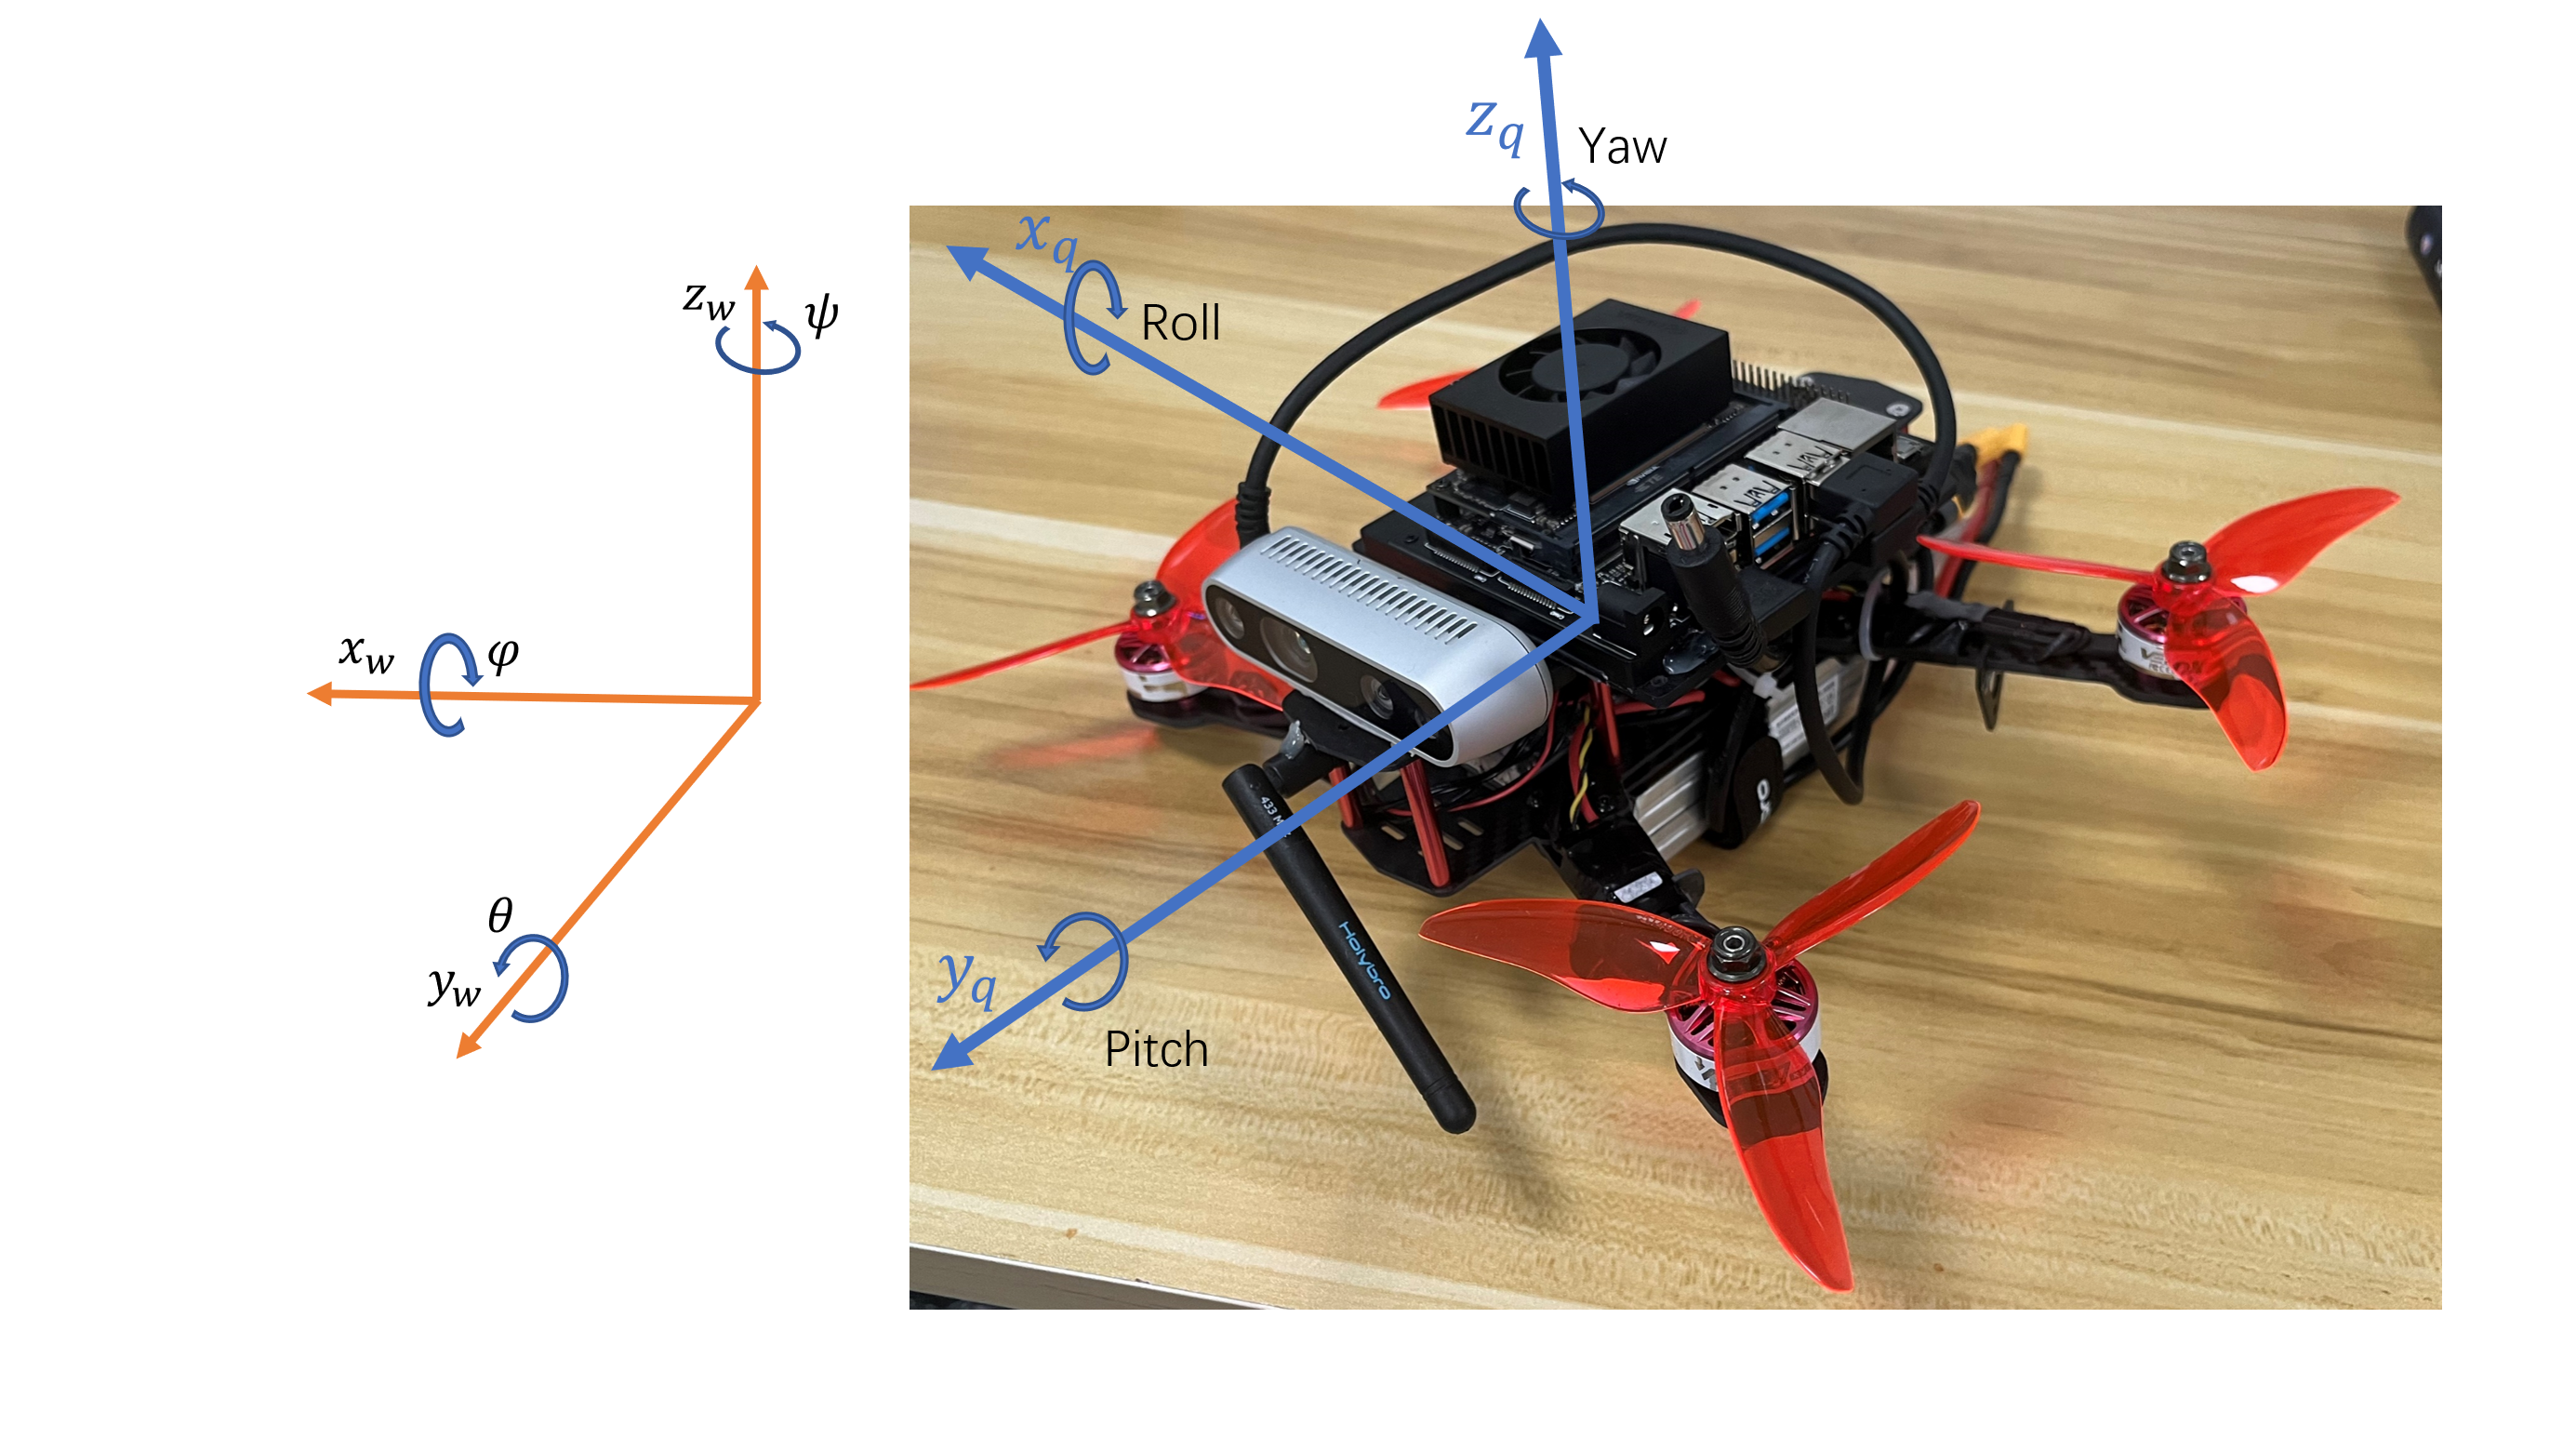
\includegraphics[width=0.7\textwidth]{coordinate.png}
      \caption{坐标系定义}
      \label{fig:1}
    \end{figure}
    首先是根据牛顿第二定律的质点动力学,由于旋翼的轴都垂直于机身平面,因此在机身坐标系下合力$f$永远垂直向下。

  \begin{equation}
    \dot x=v
  \end{equation}

  \begin{equation}
    -R \begin{bmatrix} 0\\ 0\\ f \end{bmatrix}+\begin{bmatrix} 0\\ 0\\ mg\end{bmatrix}=m \dot v 
    \label{equ:a}
  \end{equation}

    然后是刚体姿态动力学,为了表示形式的简洁以及工程实际的方便,位置和速度表示在地面系下,而角速度表示在
    机身坐标系下,因此刚体动力学方程还要加入补偿的$\omega \times J \omega$项:
  \begin{equation}
    M=J \dot\omega +\omega \times J \omega
    \label{equ:M}
  \end{equation}

    部分文献的建模中还会加入电机的陀螺力矩\cite{quanbook},$M_{gyro}=J_{rotor} \omega_{rotor} \times \omega$。 
    但出于多方面的考虑本文的模型中没有加入这一项。首先,由于控制的分层架构,在工程实现中要实时地得到电机转速  并不容易;其次,由叉乘性质可以发现,在电机转矩发生能力较弱的z轴上,陀螺力矩为$0$,其他两个方向上经过估算,
    与电机能提供的滚转俯仰力矩相比很小,完全可以当作干扰去克服;最后,省略这一项可以方便后面的理论推导。

最后是旋转矩阵导数和角速度的关系:
  \begin{equation}
    \dot R=R\Omega
    \label{equ:dotR}
  \end{equation}

\begin{proof}
  设在机身参考系下有一静止的单位向量 $r_0$ ,不妨把 $r_0$ 当作机头的方向向量,它与机体参考系固连,
  因此不随时间变化,是一个常值。其在世界坐标系下的坐标表示为 $r$ 
  $$r=R \cdot r_0$$
  
  两边对时间求导,由于 $r_0$ 是常值:
  \begin{equation}
    \dot r= \dot R \cdot r_0
    \label{equ:1}
  \end{equation}
  由于$r$是单位向量长度不变:
  \begin{equation}
    \dot r=R \omega \times r
    \label{equ:2}
  \end{equation}
  联立\ref{equ:1}  \ref{equ:2},由叉乘的分配律$A(b\times c)=(Ab)\times (Ac)$
  $$(R\omega)\times(Rr_0)=\dot R r_0$$
  $$\Rightarrow R(\omega \times r_0)=R\Omega r_0=\dot R r_0$$
  因为$r_0$任意:
  $$\Rightarrow \dot R=R \Omega'$$

\end{proof}

\subsection{动力分配}
上一节得到了从输入力和力矩到机身加速度和角加速度的关系,这一节将讨论如何从预期电机转速得到输入力和力矩。

计算单个旋翼产生的推力产生的推力和偏航力矩涉及到复杂的空气动力学,但也可以近似与转速平方成正比\cite{minimumsnap},即$f_i=k_F \omega_i^2,M_i=k_M \omega_i^2$。在正常工况的范围内,拟合较好。那么同一个旋翼产生的推力和偏航力矩就是正比关系,可以写作$M_i=c_{\tau f}f_i$。由于桨叶旋转会产生反方向力矩这一特性,如果无人机的四个旋翼全部顺时针旋转,这就会使得无人机在悬停时顺时针自转,并且无法通过控制反方向自转,逆时针同理。因此需要将无人机的桨叶配置成两正两反,对角的为一组,这样就能对消偏航力矩。在实践中,系数$c_{\tau f}$往往会非常小,这会使得控制偏航角变得困难,因有些无人机在设计时会给电机轴与机身垂直方向留出$3\sim5^\circ$的倾角,以便于改变偏航力矩。

在无人机的四个旋翼都竖直向下的情况下,无法产生水平方向的力,因此能产生的力的效果可以只用\ref{equ:trans}中等号左侧的四个参数就能表示。而旋翼的数量也是四个,这就使得动力分配变成了一一映射。分配矩阵是$4\times 4$ 的可逆方阵。
\begin{equation}
  \begin{bmatrix}
    f \\
    M_1 \\
     M_2\\M_3
    \end{bmatrix}=\begin{bmatrix}
    1 &1  & 1 & 1 \\
    0 & -d & 0 & d \\
    d & 0 & -d & 0 \\
    -c_{\tau f} & c_{\tau f} & -c_{\tau f} & c_{\tau f} \\
    \end{bmatrix}\begin{bmatrix}
     f_1\\
    f_2 \\
     f_3\\f_4
    \end{bmatrix}   
    \label{equ:trans}
\end{equation}

在得到每个旋翼的期望推力后,可以通过平方正比的关系解出期望转速,
电机速度闭环?好像不是,就是pwm开环,具体还要去看px4代码,先跳过

在仿真中,转速动态近似为一阶惯性环节,不考虑电调之类
先跳过



\section{高阶全驱系统理论}

高阶全驱(high-order fully actuated,HOFA)系统理论\cite{duan1},是由段广仁院士提出并完善为成体系的理论,为控制系统,尤其是处理非线性动态系统提供了新的视角。这一理论将卡尔曼提出的传统的一阶系统方法扩展到高阶情况,其中系统由二阶或更高阶的微分方程描述。大多数由基本物理定律建模的物理系统,比如牛顿第二定律、刚体动力学欧拉方程和基尔霍夫定律,自然表现为二阶系统。因此,HOFA系统理论提供了一种更自然和直接的方法来理解和控制这些系统,而不用将原本的高阶方程升维降阶到一阶的状态空间范畴里再设计控制算法。

\subsection*{关键概念}

\begin{itemize}
    \item \textbf{定义:}HOFA系统的特点是它们能够通过外部输入直接控制每个状态变量,这一特性基于全驱动属性。这个属性允许消除复杂的非线性动力学,简化控制设计并提高系统性能。
    
    \item \textbf{HOFA模型控制:}HOFA理论的一个核心概念是全驱动概念,这一概念从根本上改变了控制设计的方法。与最适合状态响应分析的状态空间表示不同,HOFA模型在控制应用中表现出色,为控制器设计提供了一条直接的路径。
    
    \item \textbf{控制设计:}HOFA方法在将系统表示为HOFA模型后,即可立即设计控制器。即使对于具有复杂非线性的系统,该模型也有效地线性化了控制过程,通过利用全驱动结构。
\end{itemize}

\subsection{应用与影响}

HOFA系统理论在机器人技术、航空航天和精密制造等多个领域有着广泛的应用。通过提供更直观和有效的控制设计方法,HOFA系统有潜力彻底改变我们分析、设计和实现控制系统的方式,以应对高阶和非线性动态。

\subsection{结论}

高阶全驱系统理论的发展标志着控制系统理论的重大进步。它不仅丰富了我们对复杂系统的理解,还提供了应对非线性和高阶动态挑战的实用工具。HOFA方法为控制系统设计提供了增强的能力,为各种工程领域的研究和应用开辟了新的途径。


